
\section{LITERATURE REVIEW}

\subsection{Historical Overview of Speech Recognition}
The concept of speech recognition started somewhere in 1940s, practically the first speech recognition program appeared in 1952 at the bell labs, that was about recognition of a digit in a noise free environment. 1940s and 1950s consider as the foundational period of the speech recognition technology, in this period work was done on the foundational paradigms of the speech recognition that is automation and information theoretic models. In the 1960s, it was able to recognize small vocabularies (order of 10-100words) of isolated words, based on simple acoustic-phonetic properties of speech sounds. The key technologies that were developed during this decade were, filter banks and time normalization methods. In 1970s the medium vocabularies (order of 100-1000 words) using simple template-based, pattern recognition methods were recognized. In 1980s large vocabularies (1000-unlimited) were used and speech recognition problems based on statistical, with a large range of networks for handling language structures were addressed. The key invention of this era were   model (HMM) and the stochastic language model, which together enabled powerful new methods for handling continuous speech recognition problem efficiently and with high performance. In 1990s the key technologies developed during this period were the methods for stochastic language understanding, statistical learning of acoustic and language models, and the methods for implementation of large vocabulary speech understanding systems. After the five decades of research, the speech recognition technology has finally entered marketplace, benefiting the users in variety of ways. The challenge of designing machine that truly functions like an intelligent human is still a major one going forward.

\subsection{Speech Recognition Overview}
Speech Recognition (SR) is the process of extracting the string of words automatically from the speech signal, by means of an algorithm. It is the ability of a machine or program to identify words and phrases in spoken language and convert them to a machine readable format. Speech recognition is a powerful tool of the information exchange using the acoustic signal. Therefore, not surprisingly, the speech signal is for several centuries the subject of research. Speech recognition is a technology that makes a computer able to capture the words spoken by a human with a help of microphone. These words are later on recognized by speech recognizer, and in the end, system outputs the recognized words which can also serve as input to the further systems to accomplish several task. Speech recognition is basically the science of talking with the computer, and having it correctly recognized. Speech recognition is getting the meaning of an utterance such that one can respond properly whether or not one has correctly recognized all of the words. ASR has always been considered as an important bridge in fostering better human to human and human to machine communication. In the past, however, speech never actually became an important modality in the human to machine communication. This is partly because the technology at that time was not good enough to pass the usable bar for most real world users under most real usage conditions, and partly because in many situations alternative communication modalities such as keyboard and mouse significantly outperform speech in the communication efficiency, restriction, and accuracy. In the recent years, speech technology started to change the way we live and work and became one of the primary means for humans to interact with some devices. This trend started due to the progress made in several key areas. First, Moor's law continues to function. The computational power available today, through multi-core processors, general purpose graphical processing units (GPUs), and CPU/GPU clusters, is several orders of magnitude more than that available just a decade ago. This makes training of more powerful yet complex models possible. These more computation demanding models significantly reduced the error rates of the ASR systems. Second, we can now access to much more data than before, thanks to the continued advance of the Internet and the cloud computing. By building models on big data collected from the real usage scenarios, we can eliminate many model assumptions made before and make systems more robust. Third, mobile devices, wearable devices, intelligent living room devices, and in vehicle infotainment systems became popular. On these devices and systems, alternative interaction modalities such as keyboard and mouse are less convenient than that in the personal computers. Speech, which is the natural way of human to human communication and a skill that majority of people already have, thus becomes a more favorable interaction modality on these devices and systems.



\subsection{Human Ear and Speech Recognition}
Humans are more effective than machines at recognizing speech. This advantage for
human listeners is particularly pronounced for speech that is heard against
background noise, contains unfamiliar words or is degraded in other ways. Yet,
automatic speech recognition (ASR) systems have made substantial advances over the
past few decades and are now in everyday use by millions of people around the world.
Until the performance of automatic speech recognition (ASR)  surpasses human
performance in accuracy and robustness, we stand to gain by understanding the basic 
principles behind human speech recognition (HSR).
In this section we provide a brief explanation of how human hearing works and 
how it is modeled. We will discuss in brief the functionality of several
components and try to understand the relation of it with the speech recognition systems.

\subsubsection{Human Hearing system}

The main function of hearing system is to get information about the outside, which is
carried by pressure variations in the air, that is, sound wave. Sound waves are
generated by the movement or vibration of an object, that is, sound source. As the
vibrating object moves out and in, the nearby air molecules create a slight increase
and decrease in pressure, called condensation and rarefaction, respectively. From the
pressure variations, we perceive what the sound source is and where it comes from.
We perceive a sound wave, which is a continual time series signal, by the ears.
We also perceive three-dimensional acoustic space by the ears, mainly because the
head-related transfer function (HRTF) between a point of a sound source and
the two ear entrances has directional characteristics from the shapes of the head and
the pinna. The pinna significantly modify the incoming sound, particularly at
high frequencies, and this is important in our ability for sound localization.After 
a sound wave arrives nearby, it passes through the peripheral auditory system, 
the outer ear, middle ear, and inner ear.
\begin{figure}[h]
	\begin{center}
		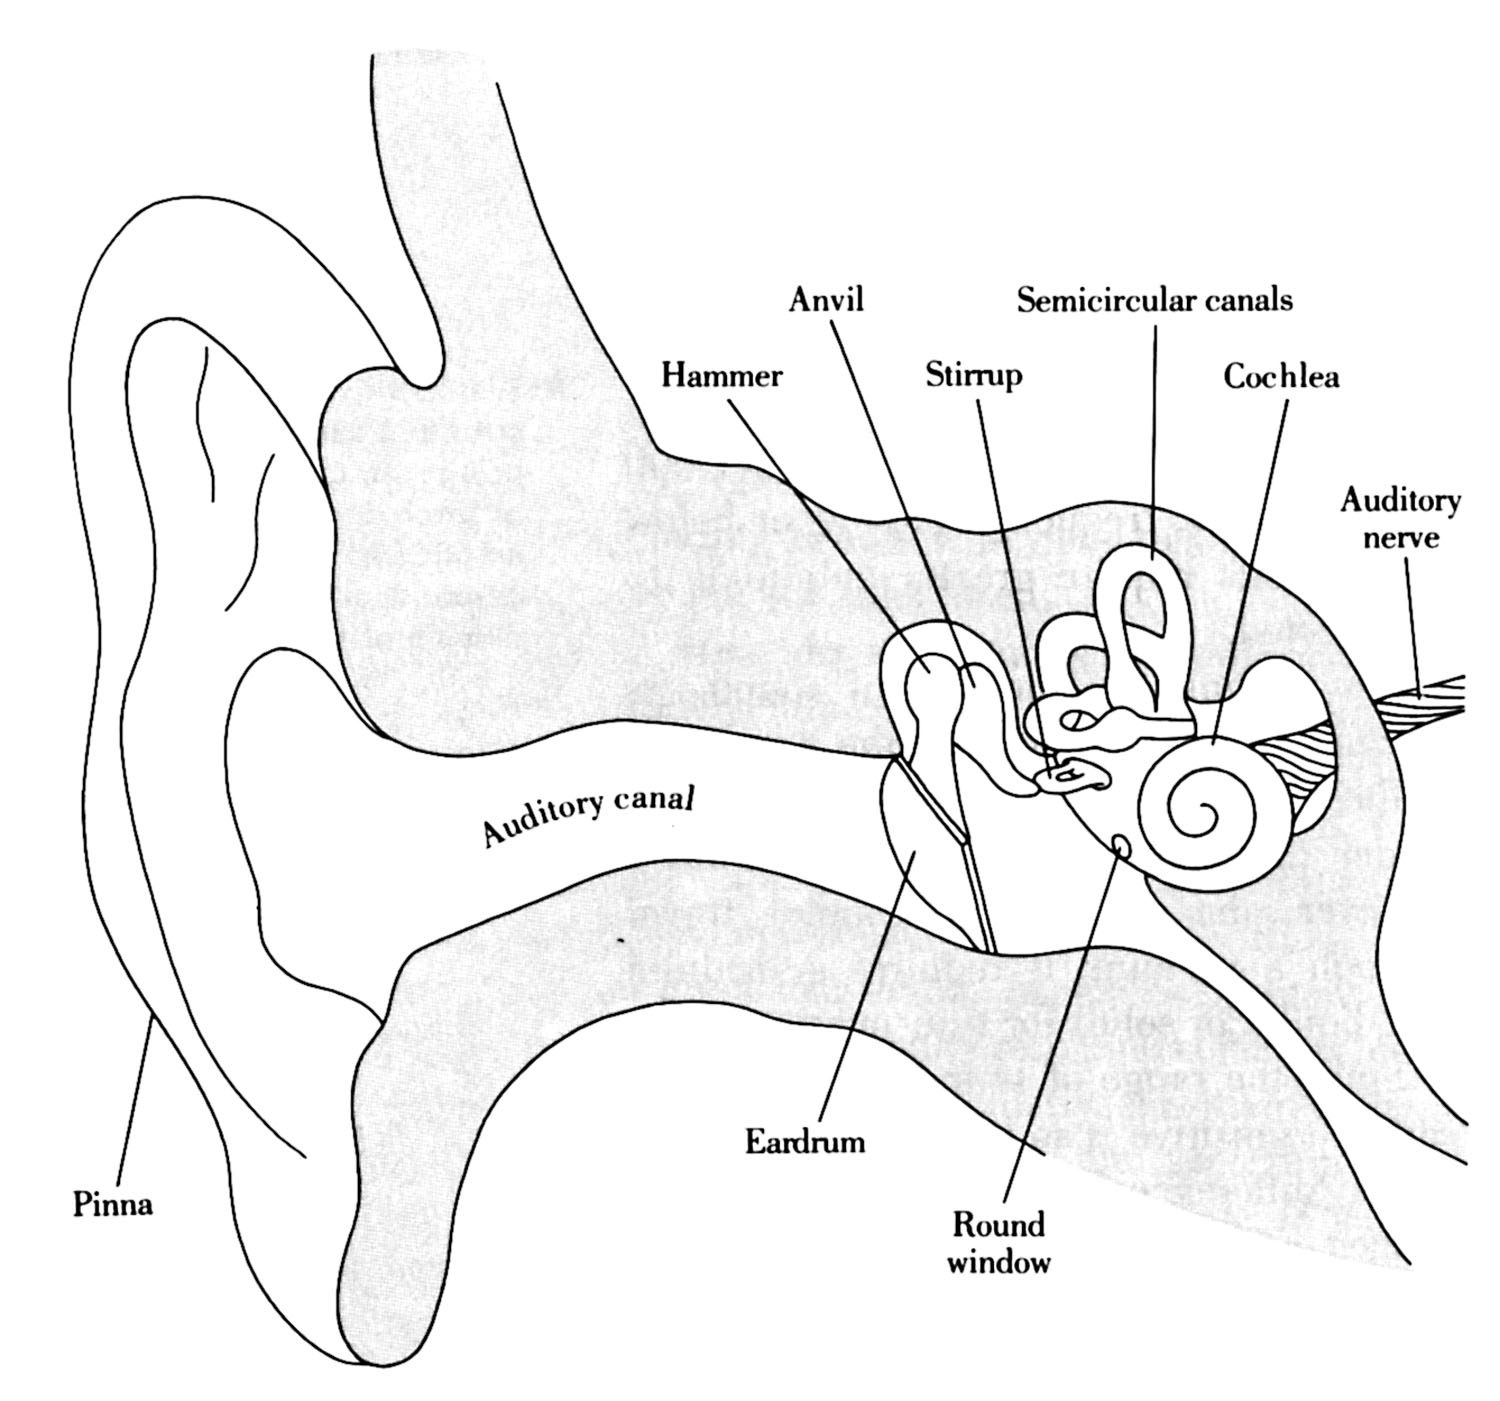
\includegraphics[scale=0.8]{images/ear_clear.jpg}
		\caption{Human Ear Hearing System}
	\end{center}
\end{figure} 

\vfill
\begin{enumerate}
	\item The Outer Ear
	
	The outer ear is the external part of the auditory system, including the pinna 
	and the ear canal. Sound travels down the ear canal and causes the eardrum, 
	or tympanic membrane, to vibrate. Because of the resonance of the outer ear, 
	we are more sensitive to sound frequencies between 1000 and 6000 Hz.
	The pinna is the only visible part of the ear (the auricle) with its special helical shape. It is the first part of the ear that reacts with sound. The function of the pinna is to act as a kind of funnel which assists in directing the sound further into the ear. Without this funnel the sound waves would take a more direct route into the auditory canal. This would be both difficult and wasteful as much of the sound would be lost making it harder to hear and understand the sounds. The pinna is essential due to the difference in pressure inside and outside the ear. The resistance of the air is higher inside the ear than outside because the air inside the ear is compressed and thus under greater pressure.
	In order for the sound waves to enter the ear in the best possible way the resistance must not be too high. This is where the pinna helps by overcoming the difference in pressure inside and outside the ear. The pinna functions as a kind of intermediate link which makes the transition smoother and less brutal allowing more sound to pass into the auditory canal (meatus).Once the sound waves have passed the pinna, they move two to three centimetres into the auditory canal before hitting the eardrum, also known as the tympanic membrane. The function of the ear canal is to transmit sound from the pinna to the eardrum. The eardrum (tympanic membrane), is a membrane at the end of the auditory canal and marks the beginning of the middle ear. The eardrum is extremely sensitive and pressure from sound waves makes the eardrum vibrate.  The auditory canal  functions as a natural hearing aid which automatically amplifies low and less penetrating sounds of the human voice. In this way the ear compensates for some of the weaknesses of the human voice, and makes it easier to hear and understand ordinary conversation.
	
	\item The Middle Ear
	
	The middle ear is the part of the ear between the eardrum and the oval window. The middle ear transmits sound from the outer ear to the inner ear. The middle ear consists of three bones: the hammer (malleus), the anvil (incus) and the stirrup (stapes), the oval window, the round window and the Eustrachian tube.The eardrum is very thin, measures approximately eight to ten millimeter in diameter and is stretched by means of small muscles. The pressure from sound waves makes the eardrum vibrate. The vibrations are transmitted further into the ear via three bones in the middle ear. These three bones form a kind of bridge, and the stirrup, which is the last bone that sounds reach, is connected to the oval window.
	The oval window is a membrane covering the entrance to the cochlea in the inner ear. When the eardrum vibrates, the sound waves travel via the hammer and anvil to the stirrup and then on to the oval window.
	When the sound waves are transmitted from the eardrum to the oval window, the middle ear is functioning as an acoustic transformer amplifying the sound waves before they move on into the inner ear. The pressure of the sound waves on the oval window is some 20 times higher than on the eardrum.
	
	
	\setlength{\parindent}{1cm}
	\setlength{\parskip}{1.1em}The pressure is increased due to the difference in size between the relatively large surface of the eardrum and the smaller surface of the oval window. The round window in the middle ear vibrates in opposite phase to vibrations entering the inner ear through the oval window. In doing so, it allows fluid in the cochlea to move. The Eustachian tube is also found in the middle ear, and connects the ear with the rearmost part of the palate. The Eustachian tube's function is to equalize the air pressure on both sides of the eardrum, ensuring that pressure does not build up in the ear. The tube opens when you swallow, thus equalizing the air pressure inside and outside the ear.
	
	\item The Inner Ear
	
	The inner ear is the innermost part of the ear, which consist of the cochlea, the balance mechanism, the vestibular and the auditory nerve. Once the vibrations of the eardrum have been transmitted to the oval window, the sound waves continue their journey into the inner ear. The inner ear is a maze of tubes and passages, referred to as the labyrinth. In the labyrinth can be found the vestibular and the cochlea.
	
	
	In the cochlea, sound waves are transformed into electrical impulses which are sent on to the brain. The brain then translates the impulses into sounds that we know and understand.The cochlea resembles a snail shell or a wound-up hose and is filled with a fluid called perilymph and contains two closely positioned membranes. These membranes form a type of partition wall in the cochlea. However, in order for the fluid to move freely in the cochlea from one side of the partition wall to the other, the wall has a little hole in it (the helicotrema). This hole is necessary, in ensuring that the vibrations from the oval window are transmitted to all the fluid in the cochlea.
	
	
	The auditory nerve is a bundle of nerve fibres that carry information between the cochlea in the inner ear and the brain. The function of the auditory nerve is to transmit signals from the inner ear to the brain.The hair fibres in the cochlea are all connected to the auditory nerve and, depending on the nature of the movements in the cochlear fluid, different hair fibres are put into motion. When the hair fibres move they send electrical signals to the auditory nerve which is connected to the auditory centre of the brain. In the brain the electrical impulses are translated into sounds which we recognise and understand. As a consequence, these hair fibres are essential to our hearing ability. Should these hair fibres become damaged, then our hearing ability will deteriorate.
	
	
	The vestibular is another important part of the inner ear. The vestibular is the organ of equilibrium. The vestibular's function is to register the body's movements, thus ensuring that we can keep our balance. The vestibular consists of three ring-shaped passages, oriented in three different planes. All three passages are filled with fluid that moves in accordance with the body's movements. In addition to the fluid, these passages also contain thousands of hair fibres which react to the movement of the fluid sending little impulses to the brain. The brain then decodes these impulses which are used to help the body keep its balance.
	
\end{enumerate}


\subsubsection{Sound Signal Transduction Mechanism}

In the human ear the basiliar membrane is contained within cochlea that supports thousands of sensory cells which forms the cochlear nerve. It is one of the innermost part of the ear. The basiliar membrane acts as a frequency spectrum analyzer. When exposed to a high frequency signal, the basilar membrane
resonates where it is stiff, resulting in the excitation of nerve cells close to the oval window.
Likewise, low frequency sounds excite nerve cells at the far end of the basilar membrane. This
makes specific fibers in the cochlear nerve respond to specific frequencies. This organization
is called the place principle, and is preserved throughout the auditory pathway into the brain. Also the principle called volley principle is used for the transduction purpose of the sound signal arriving the human ear. Here a nerve cell on the basilar membrane can encode audio information by producing an action potential in response to each cycle of the vibration. For example, a 200 hertz sound wave can be represented by a neuron producing 200 action potentials per second. However, this only works at frequencies below about 500 hertz, the maximum rate that neurons can produce action potentials. The human ear overcomes this problem by allowing several nerve cells to take turns performing this single task. For example, a 3000 hertz tone might be represented by ten nerve cells alternately firing at 300 times per second. This extends the range of the volley principle to about 4 kHz, above which the place principle is exclusively used.

\begin{figure}[h]
	\begin{center}
		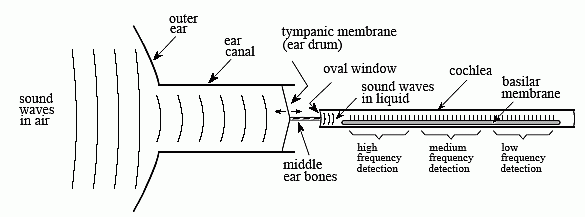
\includegraphics[scale=0.8]{images/human.png}
		\caption{Human Auditary System}
	\end{center}
\end{figure}



Table  below  shows the relationship between sound intensity and perceived loudness. It is common to express sound intensity on a logarithmic scale, called decibel SPL (Sound Power Level). On this scale, zero dB SPL is a sound wave power of $10^{-16} watts/cm2$, about the weakest sound detectable by the human ear. Normal speech is at about 60 dB SPL, while painful damage to the ear occurs at about 140 dB SPL.

\begin{figure}[h]
	\begin{center}
		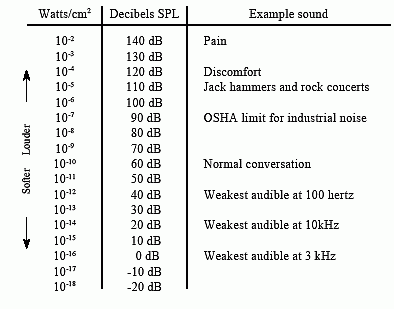
\includegraphics[scale=0.8]{images/intensity.png}
		\caption{Audibility range of sound by human ear at different 
			intensity level}
	\end{center}
\end{figure}

The difference between the loudest and faintest sounds that humans can hear is about 120 dB, a range of one-million in amplitude. Listeners can detect a change in loudness when the signal is altered by about  one dB (a 12 per cent change in amplitude). In other words, there are only about 120 levels of loudness that can be perceived from the faintest whisper to the loudest thunder. The sensitivity of the ear is amazing; when listening to very weak sounds, the ear drum vibrates less than the diameter of a single molecule.
The perception of loudness relates roughly to the sound power to an exponent of 1/3. For example, if you increase the sound power by a factor of ten, listeners will report that the loudness has increased by a factor of about two ($10^{1/3}\approx 2$). This is a major problem for eliminating undesirable environmental sounds, for instance, the beefed-up stereo in the next door apartment. Suppose you diligently cover 99 per cent of your wall with a perfect soundproof material, missing only one per cent of the surface area due to doors, corners, vents, etc. Even though the sound power has been reduced to only 1 per cent of its former value, the perceived loudness has only dropped to about 0.011/3 $\approx$ 0.2, or 20 per cent. 
The range of human hearing is generally considered to be 20 Hz to 20 kHz, but it is far more sensitive to sounds between one kHz and four kHz. For example, listeners can detect sounds as low as 0 dB SPL at three kHz, but require 40 dB SPL at 100 hertz (an amplitude increase of 100). Listeners can tell that two tones are different if their frequencies differ by more than about 0.3 per cent at three kHz. This increases to three percent at 100 hertz. 
The primary advantage of having two ears is the ability to identify the direction of the sound. Human listeners can detect the difference between two sound sources that are placed as little as three degrees apart, about the width of a person at 10 meters. This directional information is obtained in two separate ways. First, frequencies above about one kHz are strongly shadowed by the head. In other words, the ear nearest the sound receives a stronger signal than the ear on the opposite side of the head. The second clue to directionality is that the ear on the far side of the head hears the sound slightly later than the near ear, due to its greater distance from the source. Based on a typical head size (about 22 cm) and the speed of sound (about 340 meters per second), an angular discrimination of three degrees requires a timing precision of about 30 microseconds. Since this timing requires the volley principle, this clue to directionality is predominately used for sounds less than about one kHz. 
Both these sources of directional information are greatly aided by the ability to turn the head and observe the change in the signals. An interesting sensation occurs when a listener is presented with exactly the same sounds to both ears, such as listening to monaural sound through headphones. The brain concludes that the sound is coming from the center of the listener's head.
While human hearing can determine the direction a sound is from, it does poorly in identifying the distance to the sound source. This is because there are few clues available in a sound wave that can provide this information. Human hearing weakly perceives that high frequency sounds are nearby, while low frequency sounds are distant. This is because sound waves dissipate their higher frequencies as they propagate long distances. 







\subsection{Speech Recognition System}
The idea behind speech recognition is to provide a means to
transcribe spoken words into written text. There exist many approaches to achieve this goal. The most simple technique is to build a model for every word that needs to be recognized.Speech signal primarily conveys the words or message being spoken. Area of speech recognition is concerned with determining the underlying meaning in the utterance. Success in speech recognition depends on extracting and modeling the speech dependent characteristics which can effectively distinguish one word from another. The system is a collection of several modules as shown in Figure 2.4.
\begin{figure}
	\begin{center}
		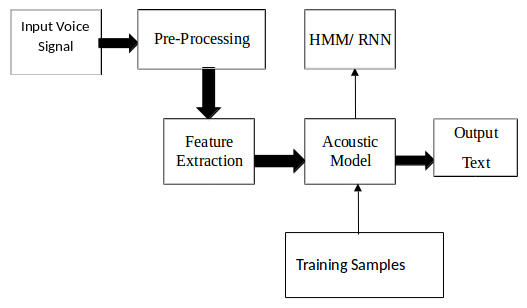
\includegraphics[scale = 0.8]{images/ASR.png}
		\caption{Speech Recognition System}
	\end{center}
\end{figure}

\subsubsection{Input Voice Signal}
The preliminary requirement of the IVR system is the input voice signal from the user such that the system may interact with the user. Most computer systems have the built in microphone facility for this purpose. Also with the help of external microphone the voice signal can be input to the system, the PC sound card produces the equivalent digital representation of received audio. During the phase of training the speech engine the recorded audio is taken and then are used for the sample generation and finally fed into the system model for training purpose and for the interactive voice response system the real time input voice of the system user is taken using the microphone. The circumstances under which input voice signal is uttered plays important role in speech recognition i.e. the factors such as too noisy environment, wrong utterance of word etc may diminish the performance of system. Therefore the input signal must be as clear as possible for the best results possible.

\subsubsection{Preprocessing stage}
The stage of the speech preprocessing refers to the purification of the input voice signal so as to feed it into main speech recognition engine in a suitable format for best outcomes.The preprocessing stage in speech recognition systems is used in order to increase the efficiency of subsequent feature extraction and classification stages and therefore to improve the overall recognition performance. Commonly the preprocessing includes the sampling step, a windowing and a de-noising step as shown in Figure below. At the end of the preprocessing the compressed and filtered speech frames are forwarded to the feature extraction stage.These processes are discussed below in brief.
\begin{figure} [h]
	\begin{center}
		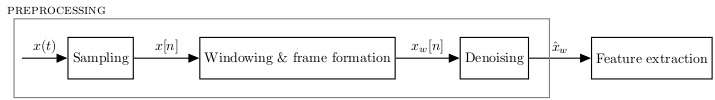
\includegraphics[scale=0.8]{images/prepro.png}
		\caption{Input speech preprocessing}
	\end{center}
\end{figure}

\begin{enumerate}
	\item Sampling stage
	
	
	In order that a computer is able to process the speech signal, it first has to be digitized. Therefore the time-continuous speech signal is sampled and quantized. The result is a time- and value discrete signal. According to the Nyquist-Shannon sampling theorem a time-continuous signal that is band limited to a certain finite frequency fmax needs to be sampled with a sampling frequency of at least $2f_{max}$. In this way it can be reconstructed by its time-discrete signal. Since human speech has a relatively low bandwidth (mostly between 100Hz and 8 KHz) a sampling frequency of 16 KHz is sufficient for speech recognition tasks. 
	
	\item Windowing and frame formation 
	
	
	Speech is a non-stationary time variant signal. We assume that human speech is built from a dictionary of phonemes, while for most of the phonemes the properties of speech remain invariant for a short period of time (~ 5-100ms). In order to obtain frames we multiply the speech signal with a windowing function. This windowing function weights the signal in the time domain and divides it into a sequence of partial signals. By doing so we gain time information of every partial signal keeping in mind that an important step of the preprocessing and feature extraction is a spectral analysis of each frame. 
	\item Denoising stage
	
	
	The stage of denoising or noise reduction, also referred to as enhancing of speech degraded by noise, aims to improve the speech signals quality. The objective is to improve the intelligibility, a measure of how comprehensible speech is. Noise corrupting speech signals can be grouped coarsely into the following three classes: 
	\begin{itemize}
		\item Microphone related noise 
		\item Electrical noise (e.g. electromagnetically induced or radiated noise) and
		\item Environmental noise
	\end{itemize}
	The first two types of noise can be easily compensated by training the speech recognizers on corresponding noisy speech samples, but compensating the environmental noise is not that elementary, due to its high variability. 
	
	Noise is ubiquitous in almost all acoustic environments. The speech signal, that is recorded by a microphone is generally infected by noise originating from various sources. Such contamination can change the characteristics of the speech signals and degrade the speech quality and intelligibility, thereby causing significant harm to human-to-machine communication systems. \\
	Noise detection and reduction for speech applications is often formulated as a digital filtering problem, where the clean speech estimation is obtained by passing the noisy speech through a linear filter. With such a formulation, the core issue of noise reduction becomes how to design an optimal filter that can significantly suppress noise without noticeable speech distortion. 
	
	Noise reduction is the crucial step in speech signal processing. Each signal is contained with some kind of noise in it which deteriotes the speech signal quality. 
	
	Noise reduction techniques depending on the domain of analyses like Time, Frequency or TimeFrequency/Time-Scale. 
	
	The Noise reduction methods are classified into four classes of algorithms: Spectral Subtractive, Subspace, Statistical-model based and Wiener-type. Some popular Noise reduction algorithms are, The log minimum mean square error logMMSE (Ephraim \& Malah 1985), The traditional Wiener (Scalart \& Filho 1996), The spectral subtraction based on reduced-delay convolution (Gustafsson 2001), The exception of the logMMSE-SPU (Cohen \& Berdugo 2002), The logMMSE with speech-presence uncertainty (Cohen Berdugo 2002), The multiband spectral-subtractive (Kamath \& Loizou 2002), The generalized subspace approach (Hu \&Loizou 2003), The perceptually based subspace approach (Jabloun \& Champagne 2003), The Wiener filtering based on wavelet-thresholded multitaper spectra (Hu \& Loizou 2004), Least-Mean-Square (LMS), Adaptive noise cancellation (ANC) [3], Normalized(N) LMS, Modified(M)- NLMS, Error nonlinearity (EN)-LMS, Normalized data nonlinearity (NDN)-LMS adaptation etc. 
	Among those many methods, one of the most simple and effective is the spectral subtraction method. It is quite popular method. Spectral Subtraction method, subtracts the estimated noise from the original signal to enhance the speech recognition. The noise is estimated from the original signal itself and subtracted to the original signal, which thus improves the Signal-to-Noise ratio (SNR). It is assumed that the signal is distorted by a wide-band, stationary, additive noise, the noise estimate is the same during the analysis and the restoration and the phase is the same in the original and restored signal.
	\begin{figure}[h]
		\begin{center}
			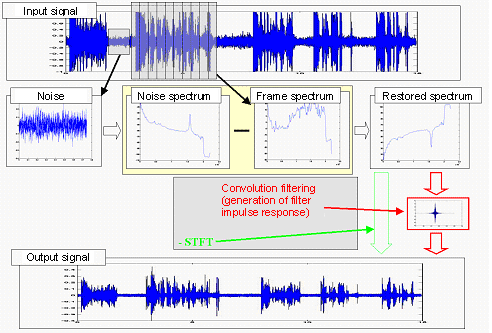
\includegraphics[scale=0.8]{images/image_2.png}
			\caption{Noise Removal Process in input voice signal}
		\end{center}
	\end{figure}
	
\end{enumerate}
\subsubsection{Feature Extraction Stage}
After the preprocessing step, feature extraction is the second component of automatic speech recognition (ASR) systems. It helps to identify the components of audio signals that are good for identifying the linguistic content and discarding all the other stuff such as background noise. The speech signal are slowly timed varying signals (quasi-stationary). When examined over a sufficiently short period of time, the characteristics of signal remain fairly stationary. The information in the speech signal is represented by the short term amplitude of the speech signal.The extraction of feature vectors is based on these short term amplitude spectrum of speech signals. This component should derive descriptive features from the windowed and enhanced speech signal to enable a classification of sounds. The feature extraction is needed because the raw speech signal contains information besides the linguistic message and has a high dimensionality. Both characteristics of the raw speech signal would be unfeasible for the classification of sounds and result in a high word error rate. Therefore, the feature extraction algorithm derives a characteristic feature vector with a lower dimensionality, which is used for the classification of sounds. 


There are several feature extraction techniques such as Linear Predictive Analysis (LPC), Linear Predictive Cepstral Coefficients (LPCC), Mel-Frequency Cepstral Coefficients (MFCC) etc. MFCC is the most commonly used feature extraction method in ASR. To extract a feature vector containing all information about the linguistic message, MFCC mimics the logarithmic perception of loudness and pitch of human auditory system and tries to eliminate speaker dependent characteristics by excluding the fundamental frequency and their harmonics. Among several features generated we consider only the relevant feature set for the classification model. These generated feature set is known as feature vector which define mathematical characteristics of a speech signal. Such feature vectors act as a input to the classification models such as HMM(Hidden Markov Mode)l, RNN(Recurrent Neural Network) etc.\\


\paragraph{Mel Frequency Cepstral Coefficients (MFCC)} \mbox{}


\textbf{Mel Frequency Cepstral Coefficients} is a popular feature extraction technique in speech recognition. The Mel Frequency Cepstral Coefficients are the representation of a windowed short term signal derived from the Fast Fourier Transform (FFT) of the signal on a non linear mel scale of frequency, which is based on the human ear scale.


For the computation of MFCC, the speech signal is divided and framed into 20-40ms long frames. The frames are overlapped for smooth transitions. The next step is to perform Discrete Fourier Transform of the frames. FFT is used to speed up the processing. Then the frequencies obtained from the FFT are wrapped onto the mel scale. A mel is a unit of pitch defined so that pairs of sounds which are perceptually equidistant in pitch are separated by an equal number of mels. The mapping between frequency in Hertz and mel scale is linear below 1000 Hz and logarithmic above 1000 Hz. The mel frequency m can be computed from frequency as 
\begin{equation}
mel(f)=1127ln(1+\frac{f}{700})
\end{equation}

The mel-spaced filterbanks are computed. This is a set of 20-40(standard is 26) triangular filters that we apply to the output of DFT from earlier steps. Then log of the each energy in the filterbank is taken. The next step is to calculate Discrete Cosine Transformation (DCT) which ranges coefficients according to the significance.

\paragraph{Linear Predictive Coding(LPC)} \mbox{}


Linear Predictive Coding (LPC) is a powerful speech analysis technique. The basic idea behind LPC is that a specific speech sample at the current time can be approximated as a linear combination of past speech samples.

Linear Prediction is the technique of computation of a parametric model based on least mean squared error theory. The speech signal is approximated as a linear combination of its precious samples. The obtained LPC coefficients describe the formants. The frequency at which the resonant peaks occur are called the formant frequencies. Thus, in this method, locations of the formants in a speech signal are estimated by computing the linear predictive coefficients over a sliding window and finding the peaks in the spectrum of the resulting LP filer.\\
\paragraph{Perceptual Linear Prediction (PLP)} \mbox{}


The Perceptual Linear Prediction model describes the psychophysics of human hearing process more accurately in feature extraction process. PLP, similar to LPC analysis, is based on the short-term spectrum of speech. But, PLP modifies the short term spectrum of the speech by several psychophysically based transformations to match human auditory system.

The PLP coefficients are calculated by first carrying out N-point DFT. A frequency warping to Bark scale is applied. The critical-band power spectrum is computed through discrete convolution of the power spectrum with the piece-wise approximation of the critical-band curve. The smoothed spectrum is down-sampled at intervals around 1 Bark. The three steps of frequency warping, smoothing and sampling are integrate into a single filter-bank called Bark filter bank. An equal loudness pre-emphasis weight the filter-bank outputs. The equalized values are further processed by Linear Prediction (LP). Applying LP to the warped line spectrum computes the predictor coefficients of a signal that has this warped spectrum as a power spectrum. 

\subsubsection{Acoustic Model}
An acoustic model is used in Automatic Speech Recognition to represent the relationship between an audio signal and the phonemes or other linguistic units that make up speech. The model is learned from a set of audio recordings and their corresponding transcripts. It is created by taking audio recordings of speech, and their text transcriptions, and using software to create statistical representations of the sounds that make up each word.


Acoustic model development is process of developing a speech recognition engine to recognize speech. The software acoustic model breaks the words into the phonemes. There are different popular ways to build this model, some of which are DTW (Dynamic Time Warping), HMM (Hidden Markov Model), RNN (Recurrent Neural Networks) etc.


\paragraph{Hidden Markov Model} \mbox{}\\

A Markov model is a stochastic model which models temporal or sequential data i.e. data that are ordered. It provides a 
way to model the dependencies of current information with previous information. The simplest Markov model is a Markov chain.
Markov Chain models the state of a system with a random variable that changes through time. In this context, the Markov property suggests that the distribution for this variable depends only on the distribution of previous state. 

\begin{minipage}{\linewidth}
	\centering
	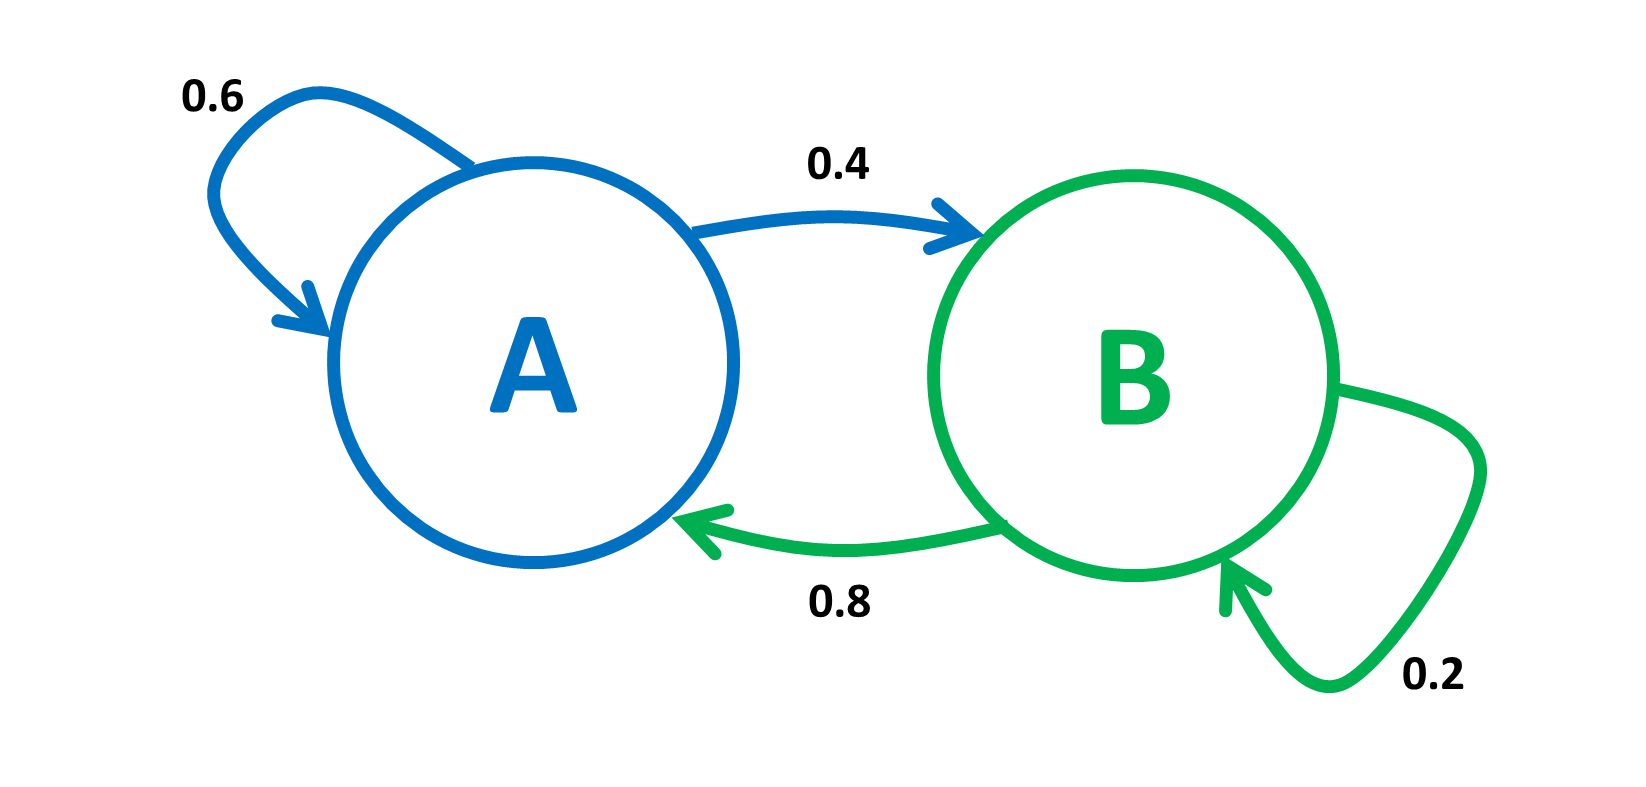
\includegraphics[scale=0.4]{markov-chain} 
	\captionof{figure}{A Markov Chain}
\end{minipage}	

A Hidden Markov Model is a Markov chain for which sate is partially observable. The observations are typically insufficient enough to precisely determine the state. A Hidden Markov Model, is a stochastic model where the states of the model are hidden. Each state can emit an output which is observed.

\begin{minipage}{\linewidth}
	\centering
	
\includegraphics[scale=0.6]{hmm} 
	\captionof{figure}{Structure of a Hidden Markov Model}
\end{minipage}	

\paragraph{Recurrent Neural Network} \mbox{}\\

A recurrent neural network (RNN) is a class of artificial neural network where connections between units form a directed cycle. This allows it to exhibit dynamic temporal behavior.

\begin{minipage}{\linewidth}
	\centering
	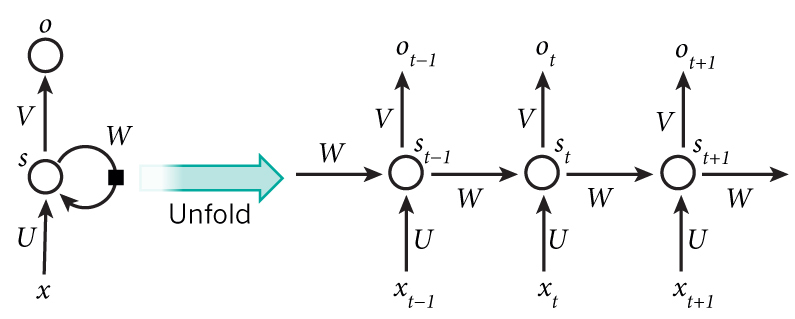
\includegraphics[scale=0.4]{rnn} 
	\captionof{figure}{A recurrent neural network and the unfolding in time}
\end{minipage}	

Recurrent networks, on the other hand, take as their input not just the current input example they see, but also what they perceived one step back in time. The decision a recurrent net reached at time step $t-1$ affects the decision it will reach one moment later at time step $t$. So recurrent networks have two sources of input, the present and the recent past, which combine to determine how they respond to new data, much as we do in life. Recurrent networks are distinguished from feedforward networks by that feedback loop, ingesting their own outputs moment after moment as input. It is often said that recurrent networks have memory. Adding memory to neural networks has a purpose: There is information in the sequence itself, and recurrent nets use it to perform tasks that feedforward networks can not.

The purpose of recurrent nets is to accurately classify sequential input. We rely on the backpropagation of error and gradient descent to do so. Recurrent networks rely on an extension of backpropagation called backpropagation through time, or BPTT. Time, in this case, is simply expressed by a well-defined, ordered series of calculations linking one time step to the next, which is all backpropagation needs to work.

Just as a straight line expresses a change in x alongside a change in y, the gradient expresses the change in all weights with regard to the change in error. If we can not know the gradient, we can not adjust the weights in a direction that will decrease error, and our network ceases to learn. Recurrent nets seeking to establish connections between a final output and events many time steps before were hobbled, because it is very difficult to know how much importance to accord to remote inputs. This is partially because the information flowing through neural nets passes through many stages of multiplication.Because the layers and time steps of deep neural networks relate to each other through multiplication, derivatives are susceptible to vanishing or exploding.

\subparagraph{LSTM RNN :} LSTM stands for Long Short Term Memory. LSTM is a variant of RNN which help preserve the error that can be backpropagated through time and layers. By maintaining a more constant error, they allow recurrent nets to continue to learn over many time steps (over 1000), thereby opening a channel to link causes and effects remotely.

LSTMs contain information outside the normal flow of the recurrent network in a gated cell. Information can be stored in, written to, or read from a cell, much like data in a computer \textquotesingle s memory. The cell makes decisions about what to store, and when to allow reads, writes and erasures, via gates that open and close. Unlike the digital storage on computers, however, these gates are analog, implemented with element-wise multiplication by sigmoids, which are all in the range of 0 to 1.

Those gates act on the signals they receive, and similar to the neural network’s nodes, they block or pass on information based on its strength and import, which they filter with their own sets of weights. Those weights, like the weights that modulate input and hidden states, are adjusted via the recurrent networks learning process. That is, the cells learn when to allow data to enter, leave or be deleted through the iterative process of making guesses, backpropagating error, and adjusting weights via gradient descent.

\begin{minipage}{\linewidth}
	\centering
	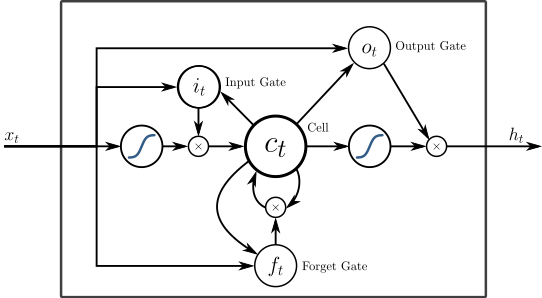
\includegraphics[scale=0.6]{LSTM} 
	\captionof{figure}{A LSTM Block}
\end{minipage}	

\subparagraph{GRU :} GRU stands for Gated Recurrent Unit. A gated recurrent unit (GRU) is basically an LSTM without an output gate, which therefore fully writes the contents from its memory cell to the larger net at each time step.

\begin{minipage}{\linewidth}
	\centering
	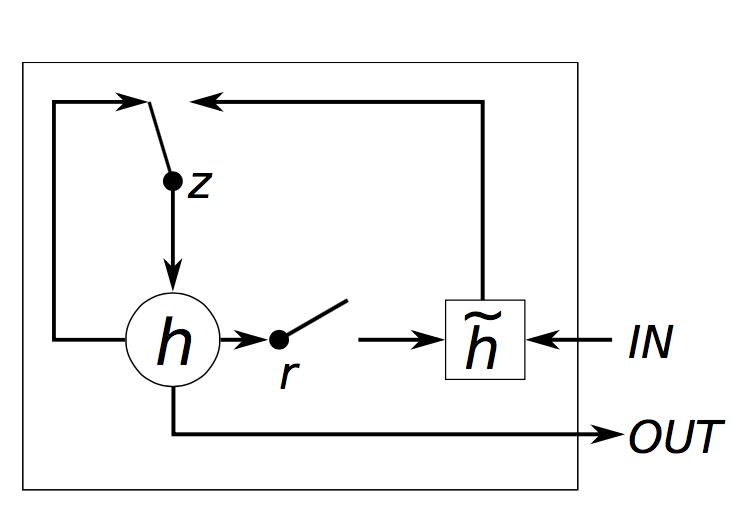
\includegraphics[scale = 0.6]{GRU} 
	\captionof{figure}{A Gated Recurrent Unit Block}
\end{minipage}	

\subsection{Types of ASR system}
Speech Recognition System are characterized by different parameters. Some of the more important of which are discussed here in brief.
\subsubsection{On the basis of input speech signal}
In Speech Recognition System the ability to recognize the speech signal can be subdivided into different classes as below:
\begin{enumerate}
	\item Isolated Words: In this type, system accepts single utterance at a time. And usually requires each utterance to have quiet on both side of sample window and require a speaker to wait between words. Its response will be better for single word but give poor result for multiple words input.
	\item Connected Words: In this type, multiple words given to the system which runs separately as isolated words and having small duration of time between them.
	\item Continuous Speech: In this type, natural speech is spoken by the user that is detectable by the machine. Continuous speech recognition is difficult to create because they utilize special method for implementation.
	\item Spontaneous Speech: In this type natural and spontaneous word has the ability to handle a variety of natural features such as words run together including mispronunciations, non-words and false statements, which are difficult to read.
\end{enumerate}
\subsubsection{On the basis of speaker model}
Every speaker has unique properties which affects the voice. On the basis of these properties system is divided into two main classes.
\begin{enumerate}
	\item Speaker Dependent Model:Speaker dependent model depends on specific speaker. These models are easier to implement and less expensive. It gives more accurate result for specific speaker and less accurate result for other speakers
	\item Speaker Independent Model:Speaker independent models depend upon many speakers. These models are difficult to implement and more expensive. It gives more accurate result for many speakers and less accurate result for specific speaker.
\end{enumerate}

\subsubsection{On the basis of type of vocabulary}
\begin{enumerate}
	\item Small size vocabulary that includes tens of words. 
	\item Medium size vocabulary that includes hundreds of words. 
	\item Large vocabulary size that includes thousands of words. 
	\item Very large size vocabulary that includes tens of thousands of words.
	\item Out of size vocabulary includes mapping a word from the vocabulary into the unknown word.
	
\end{enumerate}

\subsection{Interactive Voice Response System}

The Interactive Voice Recognition (IVR) systems through speech recognition is now enabling to go beyond the touch-tone interface models. In an IVR system, an automated message or greeting is played by the system to the caller/user. The user then responds the automated message with particular speech (voice) which is when processed through the speech processing system, outputs the corresponding speech in the text format. Now, the generated text is to be processed to make the system choose the reasonable next message or sequence of task to be followed. Then, the system selects the message (text or recorded speech) and again outputs the selected speech message back to the caller/user. This process continues on until the user/caller is transferred to a human agent or the connection is terminated. 

A system is needed on the receiving end to perform all these automated tasks. The system implements following steps to make a specific Interactive voice response system
in order to carry out its task as per the command from the user given to the system: 

\subsubsection{SoftPhone}
Softphone is basically just a part of the system which has same functions as an ordinary telephones. The IVR should be able to receive calls coming from other telephones/devices. It just handles the incoming calls. 
\subsubsection{Call Handler}
Then, a call handler is used to manage those incoming calls. This presents the caller with the auto generated voice greeting message through the speaker which then offers the selectable menu items. The caller responds to that menu through speech. 
Call handler is actually, a super set to the speech recognition system which carries out entire task of converting speech to the text. 

After the text is generated, it should be able to process the text into equivalent operations. For that the system, takes thus converted text as input and performs a search throughout the database and selects a match. During selection of a match, there arises three different cases:
\begin{itemize}
	\item Call forwarding/transferring
	
	User/Caller may ask to transfer the call to any human agent. 
	\item Automated Response Reply 
	
	
	The user might have certain queries to the system which is in the knowledge base of the system. 
	
	\item Call Termination 
	
	
	User/Caller may terminate the call after finishing their queries. 
	
	
	
	Now, in the case of the response reply, the system has to convert the selected text message back to the speech which is done by the text-to-speech module of the system and reply back to the user/caller. 
\end{itemize}






